%%%%%%%%%%%%%%%%%%%%%%%%%%%%%%%%%%%%%%%%%
% University Assignment Title Page 
% LaTeX Template
% Version 1.0 (27/12/12)
%
% This template has been downloaded from:
% http://www.LaTeXTemplates.com
%
% Original author:
% WikiBooks (http://en.wikibooks.org/wiki/LaTeX/Title_Creation)
%
% License:
% CC BY-NC-SA 3.0 (http://creativecommons.org/licenses/by-nc-sa/3.0/)
% 
% Modified for COSC480/490 by: Louis Whitburn
% Lech Szymanski (8/3/18)

\documentclass[12pt]{article}
\usepackage{cosc4x0style}

\usepackage{listings}

\usepackage{biblatex}

\usepackage{xcolor}

% Encoding goodness that I usually expect to rely on...
\usepackage[T1]{fontenc}
\usepackage[utf8]{inputenc}

\definecolor{codegreen}{rgb}{0,0.6,0}
\definecolor{codegray}{rgb}{0.5,0.5,0.5}
\definecolor{codepurple}{rgb}{0.58,0,0.82}
\definecolor{backcolour}{rgb}{0.95,0.95,0.92}

\lstset{
	backgroundcolor=\color{backcolour},   
	commentstyle=\color{codegreen},
	keywordstyle=\color{blue},
	numberstyle=\color{codegray},
	stringstyle=\color{codepurple},
	breaklines=true,
	breakatwhitespace=true,
	numbers=left,
	basicstyle=\ttfamily\small
}
 
\usepackage{amssymb}
\usepackage{amsmath}

\usepackage{graphicx}

\usepackage{wrapfig}

\addbibresource{bibliography.bib}

% The sorts of macros that I (Dave) normally use when working with LaTeX
\newcommand{\note}[2][red]{\textcolor{#1}{#2}}
\newcommand{\notedme}[1]{\note[blue]{[<Dave> #1]}}
\newenvironment{scaffold}{\color{red}}{}
\newcommand{\change}[2][]{\textcolor{orange}{#2}}

% To compile the final version of the report (which will remove all the todo content)
%\usepackage{cosc4x0style}

% Specify project code 480 or 490
\papercode{490}

% Your project title
\title{Kalman Filtering in Verilog}

% Your name
\author{Louis \textsc{Whitburn}}
\studentid{2548261}

% Names of your supervisors, separated by line break '\\'
\supervisors{
	Dr.\@ David \textsc{Eyers} \\
  	Dr.\@ Tim \textsc{Molteno}
}

% Date, change the \today to a set date if you want to be precise
\reportdate{\today}

\begin{document}


\maketitle

\begin{abstract}

With the surge in growth of the UAV (unmanned aerial vehicle) and smartphone industry, there continues to be significant demand for accurate and low power methods to measure and estimate physical orientation. The simplest method of estimating a device's orientation is by comparing the device's orientation to gravity, i.e.\@ by using accelerometers. This method is very easy to implement, however it becomes very inaccurate when the device is actually accelerating. To improve accuracy while the device is accelerating we can combine measurements from multiple sensors---such as gyroscopes and magnetometers---to calculate a more accurate estimate. This process is called ``sensor fusion'', and one of the most well known methods for performing sensor fusion is the Kalman filter. Unfortunately, the Kalman filter requires some fairly computationally expensive matrix mathematics, which limits potential performance, and results in greater than necessary power drain, when implemented in software. The existing software implementations are usually sufficient for their specific applications, however improving performance is always beneficial, and lowering power consumption is very important in devices that require recharging, such as mobile phones. My project explores the implementation of the required matrix mathematics for the Kalman filter in hardware, and the tradeoffs between hardware resource consumption and performance. One useful aspect when working with a hardware design, as opposed to a software design is the significant flexibility available for representing numerical quantities, thus I also seek to investigate how the choices of representation affect the accuracy of the inferred orientation.

\end{abstract}

\section{Introduction}

Physical orientation estimation is critical in devices such as cell phones, for example, to determine whether to orient the display in landscape or portrait. While the sales of cell phones may have slowed down in recent years, the industry is still very strong, with over one billion units sold per year \cite{Mongardini_2020}. The smartphone market is only one example of an area that requires accurate orientation data to operate correctly, e.g.\@ for augmented reality applications. State estimation using the Kalman filter is still considered the ``go-to'' approach to solving this problem, due to its simplicity and good performance, however many solutions continue to do this mostly in software \cite{ayub_2012}. This isn't ideal from an efficiency standpoint, since software implementations---while being very flexible---are not particular power efficient or fast. This is simply because modern CPUs can only run one instruction at a time, per core or pipeline. Most of the advancements in modern CPU performance have been about getting around that limit either by increasing the clock speed or reducing the amount of clock cycles it takes to execute an instruction on average (the ``single-threaded" performance), or with technologies such as SMT, SIMD instructions (such as AVX), branch prediction\footnote{Which turned out to cause more problems than it solved with meltdown and spectre} (the ``multi-threaded" performance). These technologies introduce complexity into the CPU architectures, contributing to greater power use. Several hardware-based approaches have been developed, however they are either too complex \cite{mills_2016} to be synthesised to a cheap FPGA, or are encumbered with intellectual property restrictions\footnote{Such as this one from Altera: \url{https://www.intel.com/content/dam/www/programmable/us/en/pdfs/literature/ds/extended_kalman_filter.pdf}}. I aim to produce a design that can be synthesised to any FPGA that is of a reasonable size, and interface it with sensors to give an estimate of orientation.

The primary motivation behind moving from a software implementation to a hardware implementation is reduced power consumption, although there will be an increase in performance as well. Most software Kalman filter implementations are already ``good enough'', i.e.\@ the reported data is sufficiently accurate for their application's target domain, however there is always the potential to do better, in terms of precision of the output data, or the frequency in which the system is updated. In addition, an increase in performance could be used to justify lowering the data input frequency, which would further lower power consumption. Moving the Kalman filter to hardware would also increase flexibility, allowing the CPU cycles that were used running the Kalman filter in software to do more useful work.

\section{Background}

I would like to start by introducing the Kalman filter and Hardware Description Languages (HDLs), to give some background to my project. I would also like to comment on the typical differences between software and hardware solutions to problems in order to give some context for why hardware implementations tend to perform better (i.e.\@ lower power consumption, and faster execution) than software implementations.

\subsection{Inertial Measurement Units}

An inertial measurement unit is a device which reports the acceleration and angular velocity of an object, typically by using accelerometers and gyroscopes. When combined with post-processing they can also report on the device's orientation. One method for integrating multiple sources and updating the understanding of the system is through sequential inference.

\subsubsection{Sequential Inference}

Sequential inference \cite{morrison_2016} is the process of repeatedly adding information to a model of a system to improve our understanding of the state that system is in. In particular, we can derive \cite{morrison_2016}

\begin{equation}
	\label{si}
	P(S | D_k, m) = {P(D_k | S, m) P(S | m) \over P(D_k | m)}
\end{equation}

\noindent where $S$ is the state, $D_k$ are the measurements at time step $k$, and $m$ is the model. What this equation is saying is that probability of the system being in some state, given some measurements and a model, is the product of the probability of making some measurement, given the state and the model, weighted by the ratio between the probability of being in that state (given a model of the system) and the probability of making those measurements (given a model of the system). This is simply an application of Bayes' Theorem:

\begin{equation}
	P(A | B) = {P(B|A) P(A) \over P(B)}
\end{equation}

The significance of being based off of Bayes's Theorem is that it means that equation \ref{si} can be composed to give:

\begin{equation}
	P(S|D_{k+1},D_k,m) = {P(D_{k+1}|D_k,S,m) \over P(D_{k+1}|D_k,m)} P(S | D_k, m)
\end{equation}

\noindent Thus we can add more measurements to our system to gain a better understanding of the state that it is in. Sequential Inference provides the theoretical bases for the Kalman Filter---one of the most widely used applications of sequential inference---which I discuss below.

\subsubsection{Kalman Filter}

The Kalman filter \cite{kalman_1960} is one of the most popular solutions for estimating the state (e.g.\@ orientation) of a system from multiple noisy sensors, due to its relative simplicity while still performing optimally\footnote{Here, optimally refers to how the calculated ``Kalman gain'' minimises the ``post-fit residual'', which is discussed later in this section.} \cite{wangyan_2015}. It works by using a model of the system to predict the future state of that system, and then (after some time step), comparing that predicted state to the measured state.

The first two steps are to predict how the system will evolve:
\begin{eqnarray}
	\mathbf{\hat{x}}_{k | k-1} &=& \mathbf{F}_k \mathbf{\hat{x}}_{k-1|k-1} + \mathbf{B}_k \mathbf{u}_k \\
	\mathbf{P}_{k|k-1} &=& \mathbf{F}_k \mathbf{P}_{k-1 | k-1} \mathbf{F}^T_k + \mathbf{Q}_k
\end{eqnarray}

Here, $\mathbf{\hat{x}}_{k | k-1}$ and $\mathbf{P}_{k|k-1}$ are the \emph{a priori} (i.e.\@ without including any additional knowledge) estimates of the state, and the covariance of the state. Our \emph{a priori} knowledge comes only from the previous state---the $k-1|k-1$ subscripts. $\mathbf{F}_k$ is the state transition matrix, i.e.\@ it determines how the state changes through time. $\mathbf{B}_k$ is the control-input matrix applied to the control vector $\mathbf{u}_k$---these model any external input to the system, i.e.\@ if it was forced in a direction. Finally, $\mathbf{Q}_k$ is the covariance of the process noise, i.e.\@ the error / uncertainty that arises from the model. This uncertainty mainly arises from approximations made in the model (e.g.\@ linearisation), and from integration error (e.g.\@ if the measurement is velocity, then the estimate of position will drift if not corrected).

The next step is the update step. It first consists of the innovation stage---determining the difference between the predicted / forecast state and the observed state
\begin{eqnarray}
	\mathbf{\tilde{y}}_k &=& \mathbf{z}_k - \mathbf{H}_k \mathbf{\hat{x}}_{k|k-1} \\
	\mathbf{S}_k &=& \mathbf{H}_k \mathbf{P}_{k|k-1} \mathbf{H}^T_k + \mathbf{R}_k
\end{eqnarray}

Here $\mathbf{\tilde{y}}_k$ is that difference (residual), where $\mathbf{z}_k$ is the measured state and $\mathbf{\hat{x}}_{k|k-1}$ is the \emph{a priori} estimate from before. $\mathbf{H}_k$ is the observation model, which maps the state space into the observation space---e.g.\@ when measuring depth via sonar the state space contains the depth, whereas the observation state contains the sonar round trip time. The observation model converts this (predicted) state into a (predicted) observation, in this case by dividing the distance by half the speed of sound in water. $\mathbf{S}_k$ is the residual of the covariance, where $\mathbf{R}_k$ is the covariance of the process noise, in the above example, this could arise from water currents and temperature differences slightly affecting the speed of sound in the water. It could also arise from imprecise sensors.

The second part of the update step is determining the Kalman gain:
\begin{eqnarray}
	\mathbf{K}_k = \mathbf{P}_{k|k-1} \mathbf{H}^T_k \mathbf{S}^{-1}_k
\end{eqnarray}

\noindent This generates a gain matrix which aims to minimise the \emph{a posteriori} (updated with the sensor observations) residual, $\mathbf{\tilde{y}}_{k|k} = \mathbf{z}_k - \mathbf{H}_k \mathbf{\hat{x}}_{k|k}$.

The final part is generating these \emph{a posteriori} estimates
\begin{eqnarray}
	\mathbf{\hat{x}}_{k|k} &=& \mathbf{\hat{x}}_{k|k-1} + \mathbf{K}_k \mathbf{\tilde{y}}_k \\
	\mathbf{P}_{k|k} &=& (\mathbf{I} - \mathbf{K}_k \mathbf{H}_k)\mathbf{P}_{k|k-1}
\end{eqnarray}

\noindent where $\mathbf{\hat{x}}_{k|k}$ and $\mathbf{P}_{k|k}$ are the \emph{a posteriori} state estimate and state estimate covariance.

Thus we have a mechanism to have our estimate of the state optimally track the actual state. In the above equations, the matrices (uppercase and bold) are of the size $n \times n$ and the vectors (lowercase and bold) are column vectors of the size $n \times 1$, where $n$ is the size of the estimated state. The observation space need not be the same size as the state space, thus if the size of the observation space is $m$, then $\mathbf{H}_k$ may be $m \times n$ and $\mathbf{z}_k$ may be $m \times 1$, however I will assume that $n = m$ for simplicity.

\subsection{Naive Matrix Algorithms}
\label{naive}

For this project, the required matrix operations are:

\begin{itemize}
	\item Multiplication (by a vector or other matrix)
	\item Scaling (multiplication by a scalar)
	\item Transposition
	\item Determinant
	\item Inverse
\end{itemize}

Of these, transposition is by far the easiest, since it is nothing more than shuffling some data around. The next easiest is scaling, which can be implemented by something as simple as a loop through all of the elements of the vector or matrix, and multiplying it by the scalar. Multiplication by a vector or matrix is also comparatively simple, as it is just a series of dot products.

The two more difficult operations are the determinant and inverse. The naive matrix determinant algorithm \cite{strang2006linear} is

\begin{equation}
	\det{\mathbf{A}} = 
	\begin{cases}
	a_{11}a_{22} - a_{12}a_{21}& \mathbf{A} \in \mathbb{R}^{2 \times 2}\\
	\sum_{i=1}^{n} a_{1i}  (-1)^{i-1}\det{\mathbf{A}^{1i}} & \mathbf{A} \in \mathbb{R}^{n \times n}, n > 2\\
	\end{cases}
\end{equation}

\noindent
where $\mathbf{A}^{ij}$ means the matrix $\mathbf{A}$, but excluding row $i$ and column $j$. To give an estimate of complexity, a $4\times4$ matrix would require four $3\times3$ matrix determinants to be calculated, and each one of those would require three $2\times2$ matrix determinants to be calculated. Thus this is $\mathcal{O}(n!)$ (where $n$ is the amount of rows in the matrix), i.e.\@ very slow.

The inverse is even more complicated:
\begin{equation}
	a^{-1}_{ij} = \frac{1}{\det{\mathbf{A}}} \left(a_{ij} (-1)^{i+j} \det{\mathbf{A}^{ij}}\right)^T
\end{equation}
\noindent
and is also $\mathcal{O}(n!)$.

These are OK for small matrices, however for this project I am targeting a $12 \times 12$ matrix. Thus, assuming a $2\times2$ matrix takes one time step, a $12 \times 12$ would take $\frac{12!}{2!} \approx 2.4 \times 10^8$ time steps. This is obviously unacceptable if we expect a Kalman Filter based off of this to operate in real time\footnote{Or in any reasonable time at all. I estimated it would take a day to even simulate the $12\times12$ matrix inverse testbench. \notedme{first instance of the term `testbench'---explaining what this is should have already appeared in the body text}}.

\subsection{Better Matrix Algorithms}
\label{lu}

\notedme{Rework this paragraph. You clearly understand what's going on, so that's good. However, I'd say bring the footnote into the body text, and provide an explanation before you use the maths. E.g., you use $\mathbf{L}$ and $\mathbf{U}$ before you've said what they mean... also make a macro for transpose: you're using inconsistent forms at the moment.}
Thankfully there are better ways\footnote{This is very common with numerical methods, often the more intuitive methods are mathematically ``cleaner'', however they tend to be slower, or more numerically unstable, than the less intuitive but more optimised algorithms.}. Imagine we could factor $\mathbf{A} = \mathbf{L}\mathbf{U}$. Thus $\det(\mathbf{A}) = \det(\mathbf{L^T}) \det(\mathbf{U})$, since $\det(\mathbf{AB}) = \det(\mathbf{A}) \det(\mathbf{B})$, and $\det(\mathbf{A}^T) = \det(\mathbf{A})$. Thus,  if $\mathbf{L}$ is lower triangular (such that $\mathbf{L}^T$ is upper triangular), and $\mathbf{U}$ is upper triangular, and all the diagonal entries in $\mathbf{L}$ are $1$, then we can work out $\det{\mathbf{A}}=\sum_{i=1}^{n}u_{ii}$, since the determinant of an upper triangular matrix is just the product of the diagonal entries\footnote{The reason for this is that if--when calculating the determinant the naive way---we use the left column for the multiplication factors, as opposed to the top row, then only the upper left of each sub-determinant we have to calculate will be non-zero, thus we only have to calculate one determinant for each iteration of the recursion, and multiply it by that value on the diagonal. When we reach the base $2\times2$ case, the bottom left value will be zero, thus the determinant will be the product of the two diagonal elements. Thus as we work back from the bottom of the recursion we only ever multiply the values on the diagonal.}. This means calculating the determinant is $\mathcal{O}(n)$, which is a huge improvement.

Working out the inverse is simple. If $\mathbf{AX}=\mathbf{I}$, then we know $\mathbf{A}^{-1} = \mathbf{X}$. This is just solving $\mathbf{LUx}=\mathbf{i}$ $n$ times, where $\mathbf{x}$ is the $n$\textsuperscript{th} column of $\mathbf{X}$ and where $\mathbf{i}$ is the $n$\textsuperscript{th} column of $\mathbf{I}$. This is incredibly straightforward, since $\mathbf{L}$ and $\mathbf{U}$ are upper triangular, thus we can use forward and back substitution to solve this as two sets of simultaneous equations. This is $\mathcal{O}(n^3)$, since all three operations are linear.

Of course this all assumes that working out $L$ and $U$ is simple.

This process is called the ``LU Decomposition''\cite{lu_decomposition}. It also provides a third matrix, $\mathbf{P}$, the permutation matrix. This is because the LU decomposition is based off of Gaussian elimination, which may require swapping rows, and thus to rebuild $\mathbf{A}$ from $\mathbf{L}$ and $\mathbf{U}$ we need to know which rows were swapped, thus $\mathbf{PA}$ = $\mathbf{LU}$. The details of the LU decomposition are unimportant, beyond that it involves Gaussian elimination, however what is important to note is that the LU decomposition is $\mathcal{O}(n^3)$. Since the inversion or determinant steps come after the LU decomposition, the complexity is added, not multiplied. Thus calculating the determinant and inverse is still only $\mathcal{O}(n^3)$ i.e.\@ polynomial.

One corollary of the above is this: We can still implement the naive inverse using the better determinant. Since the naive inverse requires $n^2$ determinants (of size $n-1 \times n-1$, which is still $\mathcal{O}(n^3)$), this means that this half-naive approach is $\mathcal{O}(n^5)$. This is still significantly better than $\mathcal{O}(n!)$, and I will discuss this aspect more later in this report.

In addition to the LU decomposition there is also the QR decomposition, and the singular value decomposition (SVD)\cite{num_lin_alg}. The QR decomposition was not chosen because it is slightly slower that the LU decomposition (about twice as slow), and the SVD was not chosen because it is harder to implement, and because it is more suited to solving homogenous equations (i.e\@ those of the form $\mathbf{A}\mathbf{x}=\mathbf{0}$), or, if there is no such $\mathbf{x}$ that satisfies that equation, then it can also be used to solve the ``least-squares'' problem, where we want to find the $\mathbf{x}$ which minimises $||\mathbf{Ax}||_2$ (the 2-norm of $\mathbf{Ax}$, for a vector this will be the magnitude). This is extremely important (and with the SVD, very fast), however this is not relevant to this project.

\subsection{Hardware Description Languages}

The 1975 MOS Technology 6502 consisted of approximately 3500 transistors. This is a comprehensible size, in that it is entirely possible to imagine it being designed by hand. On the other hand, the first CPU to introduce the x86 instruction set was the Intel 8086 back in 1978, made from some 29,000 transistors. An Intel Nehalem CPU from 12 years ago contains upwards of 750 million transistors. AMD's ``Epyc'' lineup of server CPUs contain up to 50 billion transistors per CPU. These would either be difficult and time consuming to design by hand (in the case of the 8086), or downright impossible to design by hand (the modern Nehalem and Epyc Rome CPUs). Thus it was the development of Hardware Description Languages (HDLs) that enabled us to make our huge modern integrated circuits in a reliable fashion.

If I write a program in a language such as C, and target a conventional architecture, such as ARM or x86, then the code that I write is not the actual program---it only describes the program. For example, no CPUs contain a `for loop' instruction---a `for loop' in C is converted into (some variation of) a label, a comparison, and a conditional jump to the position described by that label. The process of turning the description of the program to the actual program is ``compilation'', and this is well understood.
HDLs are the hardware equivalent of high level programming language---they do not describe logic gates and how they are connected, however they describe the behaviour of the hardware in a way such that it can be ``synthesised'' to the actual logic. For example, instead of having to describe each individual gate and connection in an adder, the designer can simply type \lstinline[language=Verilog]|a + b| and the synthesiser will generate the appropriately sized adder from that.

This can of course be used for more complex problems. For example, designing a minimal\footnote{Designing a useful CPU is more complicated but entirely achievable---this one can even boot inux: \url{https://github.com/ultraembedded/biriscv}} CPU in an HDL is almost trivial---all it needs is a suitably large array (to act as memory), and a few \lstinline[language=Verilog]|if| statements to determine what to do with each opcode.

In a few hours, I was able to design such a minimal CPU\footnote{I want emphasise here just how minimal this CPU is---inefficient, doesn't support a stack, no registers, no signed integers, no floating point numbers etc.\@---it is just a toy to show what can be done with HDLs such as Verilog.} (using an HDL called ``Verilog''), in only around 150 lines of code (which is included in \ref{verilog_cpu}). This code also creates a small block of memory, into which I and in that memory some instructions. Those instructions are (in plain English):

\begin{enumerate}
	\item Set value at memory address \texttt{0xf0} to \texttt{0x10} (16).
	\item Set value at memory address \texttt{0xf1} to \texttt{0x01} (1).
	\item Output the value at memory address \texttt{0xf0} (this causes the testbench to print the number).
	\item If the value at memory address \texttt{0xf0} is 0, then jump to instruction 7.
	\item Subtract the value at memory address \texttt{0xf1} from the value at \texttt{0xf0}, and store it at \texttt{0xf0}.
	\item Jump to instruction 3.
	\item Jump to instruction 7 (this instruction, i.e.\@ halt).
\end{enumerate}

In other words, it counts down from 16 to 0. We can see this in the output from when the CPU and testbench is simulated (each line below is from instruction 3 above):

\lstinputlisting[numbers=none, backgroundcolor=\color{white}]{cpu-bench-result.txt}

In other words, it is a perfectly functioning CPU\footnote{In that it is Turing complete, apart from the finite amount of memory} with its own machine language code, which supports very basic port-mapped I/O, unconditional and conditional branching, and basic unsigned integer arithmetic---in around 150 lines of code.

\subsubsection{Icarus Verilog}

Like all code, code written in HDLs such as Verilog needs to be tested to ensure that bugs are found and fixed before the hardware is manufactured. It is entirely possible to synthesise the Verilog to an FPGA and perform the tests on the FPGA, however this is difficult to automate, since it requires interfacing with external hardware. If all we want to do is simple verification that the Verilog we wrote is correct, then we can just simulate the Verilog in software and automatically check that the code behaves as we expect.

One tool for this is Icarus Verilog (Icarus), which is available under the GNU General Public License (GPL). With Icarus, I can simply create a testbench module, and run automated tests on any Verilog code I write or generate. I used this same approach to simulate the CPU that I presented earlier---the code in the \lstinline[language=Verilog]|cpu_test| module is not synthesisable (i.e.\@ it can't be turned into an actual circuit\footnote{I'll provide more detail here. The \lstinline[language=Verilog]|cpu| module is synthesisable, since all of what it does can be mapped to actual hardware (e.g.\@ multiplexers, lookup tables, flip flops, etc.\@), however the \lstinline[language=Verilog]|cpu_test| module includes code such as displaying to a console, introducing arbitrary delays, stopping execution}), however Icarus is able to parse it and use it to simulate the \lstinline[language=Verilog]|cpu| module (which is synthesisable).

\subsection{Hardware vs.\@ Software Considerations}

Many common operations on large matrices can be defined recursively, such as the determinant of an $n \times n$ matrix being a function of the determinants of its $(n-1) \times (n-1)$ minor matrices. Recursive algorithms are fairly simple to express mathematically and can be rather intuitive, however many implementations of these recursive algorithms introduce inefficiencies, such as calculating the same value multiple times. One example of this is the Fibonacci sequence:

\begin{align}
	F_0 &= 0 \\
	F_1 &= 1 \\
	F_n &= F_{n-1} + F_{n-2}
\end{align}

\noindent Calculating $F_4$ requires knowing $F_3$ and $F_2$, but the calculation of $F_3$ also requires knowing $F_2$. This means that we need to calculate $F_2$ at least twice, which is an inefficient use of time---and we have to wait until $F_2$ is determined before we can even start to calculate $F_3$. The first problem can be solved using techniques such as memoisation, however the second problem is inherent in software, since the CPU (assuming it is something mainstream like x86 or ARM) needs to perform one instruction after another\footnote{Modern CPUs have multiple cores, and many support simultaneous multithreading, which allow some parallelism, but still nowhere near as much as even a \$5.00 dollar FPGA}, creating a dependency in time between the calculation of $F_3$ and $F_2$, as shown in figure \ref{fib_block}.

\begin{figure}[thp]
	\centering
	
	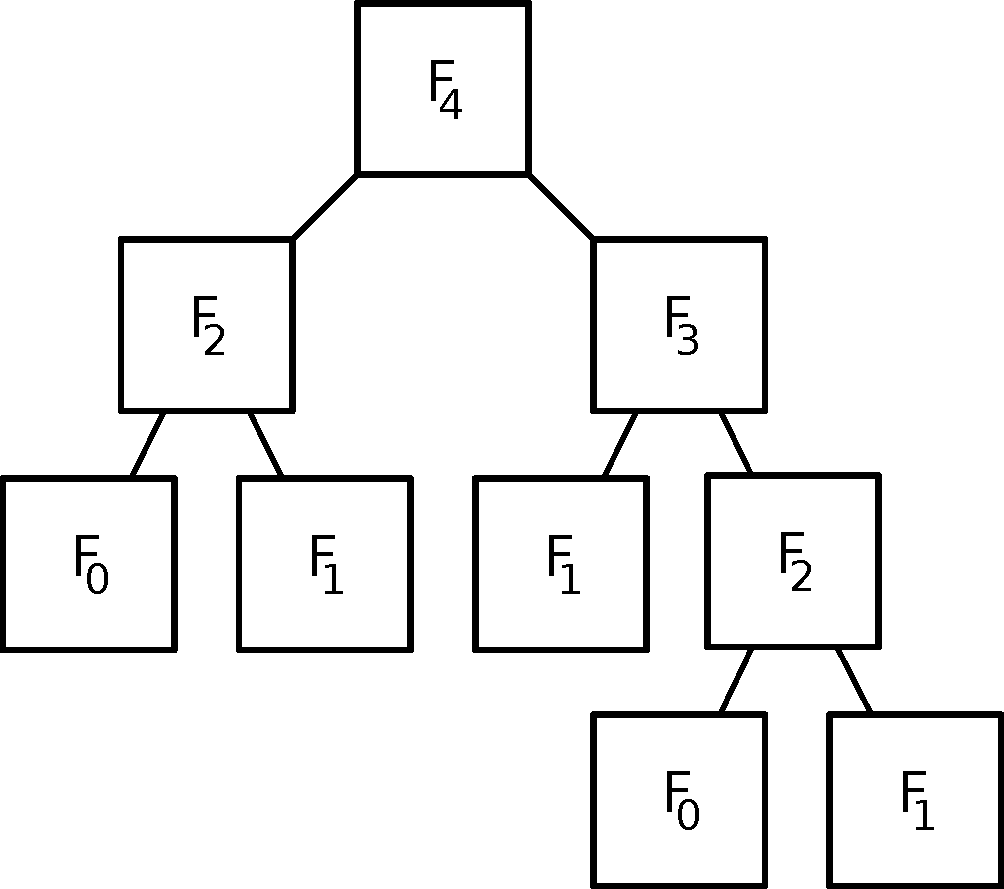
\includegraphics[width=\textwidth]{fib-block.pdf}
	
	\caption{A diagram showing the dependencies for the recursion of calculating the fourth Fibonacci number.}
	\label{fib_block}
\end{figure}

Hardware solves this problem by moving the time dependency into a spatial dependency---we can create several Fibonacci modules, and wire them into each other, e.g.\@ the $F_4$ module could take inputs from an $F_3$ module and an $F_2$ module. Since these modules act almost instantaneously this makes the overall calculation also almost instantaneous.

We can see the contrast between hardware and software in the determinant calculation described earlier. A software implementation, like the one listed in \ref{recursion_time} takes time but uses very little space, whereas the one listed in \ref{recursion_space} takes almost no time but a lot of space (and the code I present is limited to $4\times4$)---despite both being basically the same naive, recursive algorithm. Here we see the differences between hardware and software---hardware is inherently parallel, whereas software is inherently sequential. For the software side, consider multi-core CPUs. Writing programs that run in parallel is more difficult than single-threaded programs since care has to be taken to prevent contention and race conditions. For the hardware side, consider the CPU I presented earlier. Assuming I wanted to print the numbers from some value $n$ down to zero, I could simply have created a Verilog ``generator'', which would have generated the hardware to print all those numbers, similar to an unrolled for loop in a language like C.

The other advantage hardware has over software is that it can be made very specific to an application, meaning that the overhead associated with having a CPU can be removed for the specific hardware concerned. For example, a hardware Fibonacci module does not require complex instruction decoding circuitry because it only performs one operation.

\section{Progress}

\subsection{Python Kalman Filter / Test Harness Development}

The first phase of the project was getting a simple Kalman filter working. This was based on a simple one-dimensional cart moving backwards and forwards, with the measured quantity being position. In figure \ref{1d_position_fig} we can see the system handles both a fairly predictable motion as well as an unpredictable motion quite well. 
\notedme{Probably best to include a description of the experiment in the body text too, rather than relying on the caption.} \todo{as mentioned in interim report feedback, has been on my to do list}
This is to be expected since we are measuring position, thus we expect the estimate of position to be fairly accurate (for obvious reasons). The estimate of velocity slowly converges to the actual velocity, however it has to re-converge after the bump. This is also expected since the bump was modelled as an impulse, which isn't a 100\% realistic scenario.

\begin{figure}[thp]
	\centering
	
	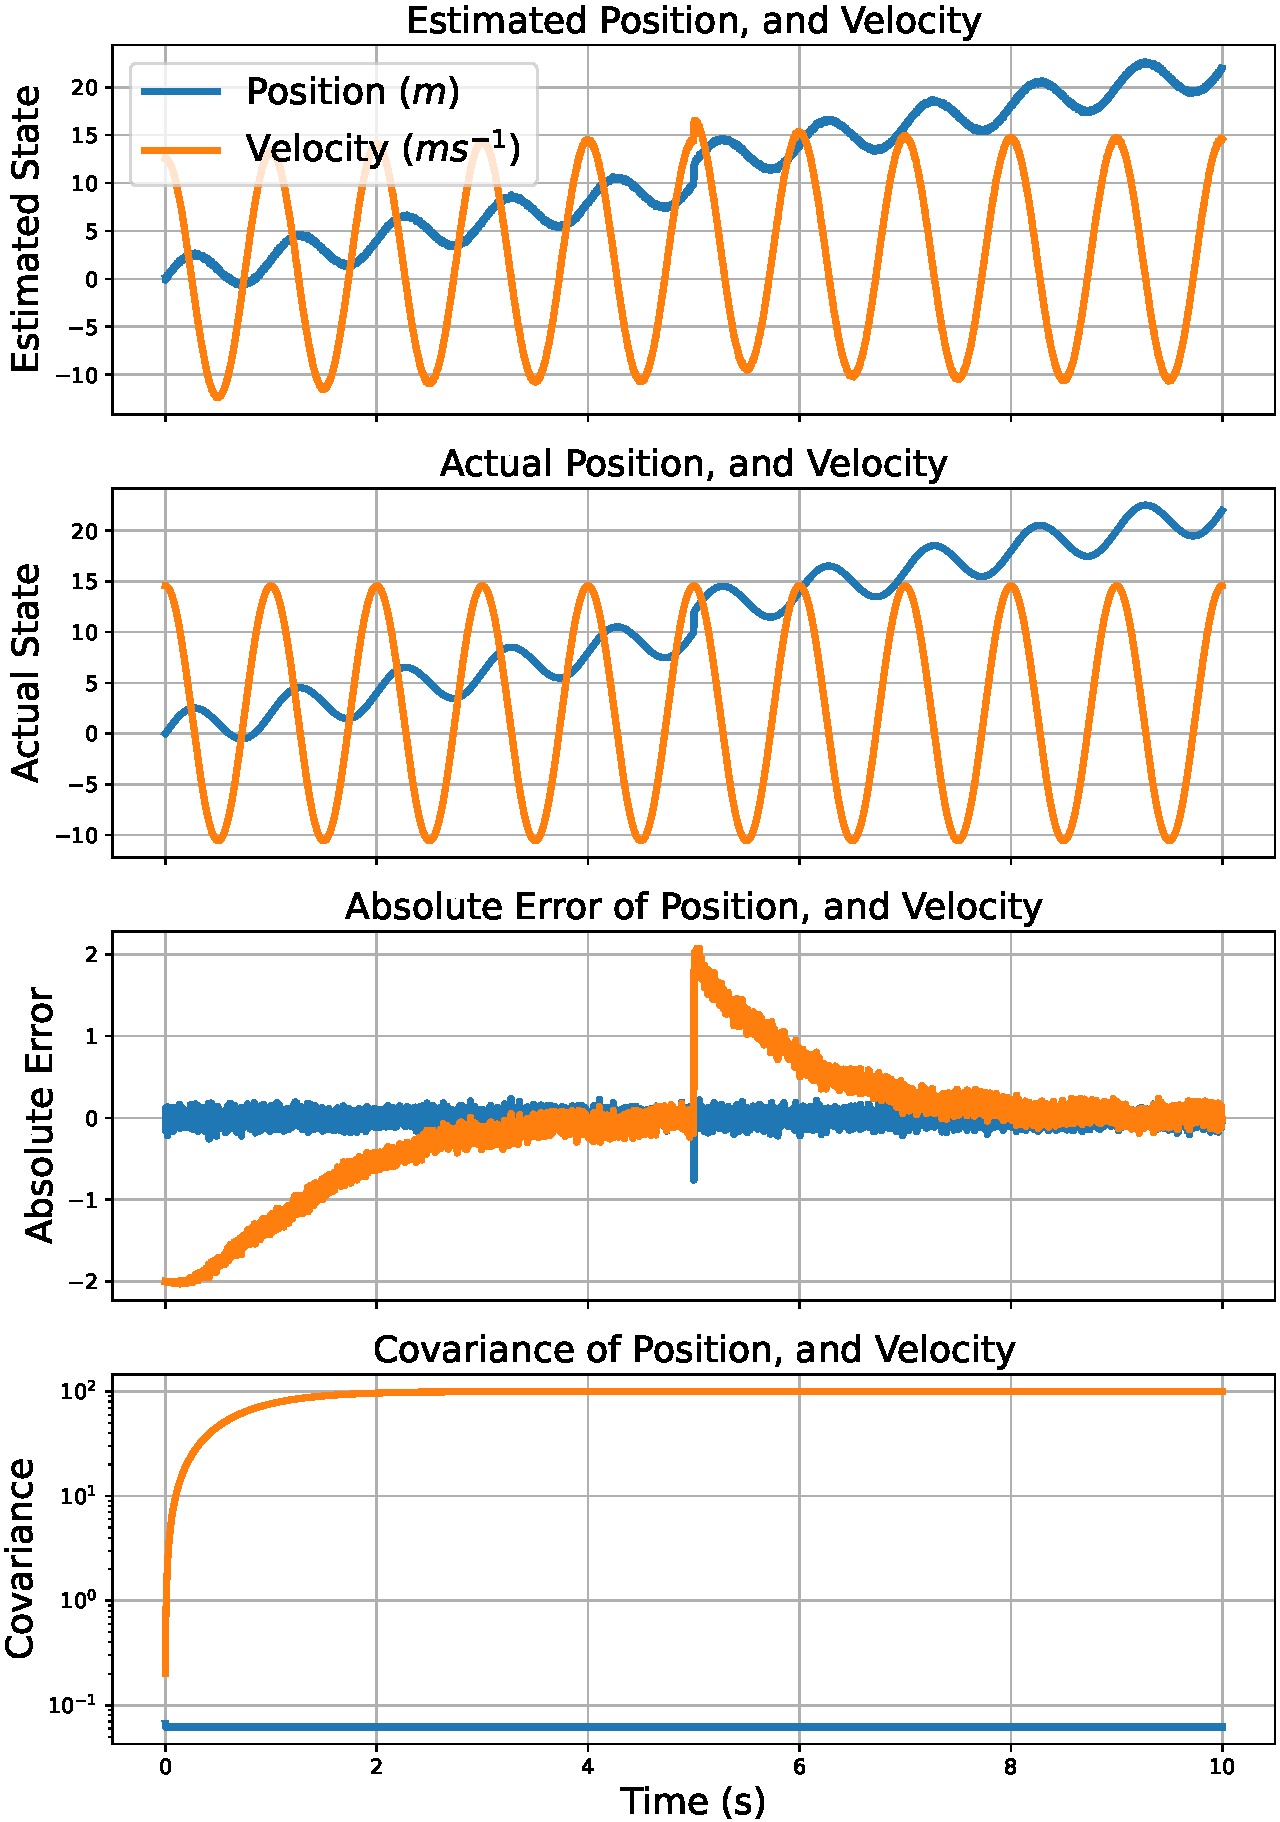
\includegraphics[height=0.8\textheight]{1d-position.pdf}
	
	\caption{A cart moving backwards and forwards, with a slight tendency to move in the positive direction. The cart is ``bumped'' at $t=5$, where we see the error of the velocity increase, until it settles down into a new equilibrium.}
	\label{1d_position_fig}
\end{figure}

The next system was the same as before except the velocity was measured, and the position determined by integrating---i.e.\@ by adding the velocity multiplied by the time step to the previous position. In this scenario, the velocity is cyclical, with a slight increase over time. As we can see in figure \ref{1d_velocity_fig}, the model continues to perform well, with minimal error which appears to be bounded.

\begin{figure}[thp]
	\centering
	
	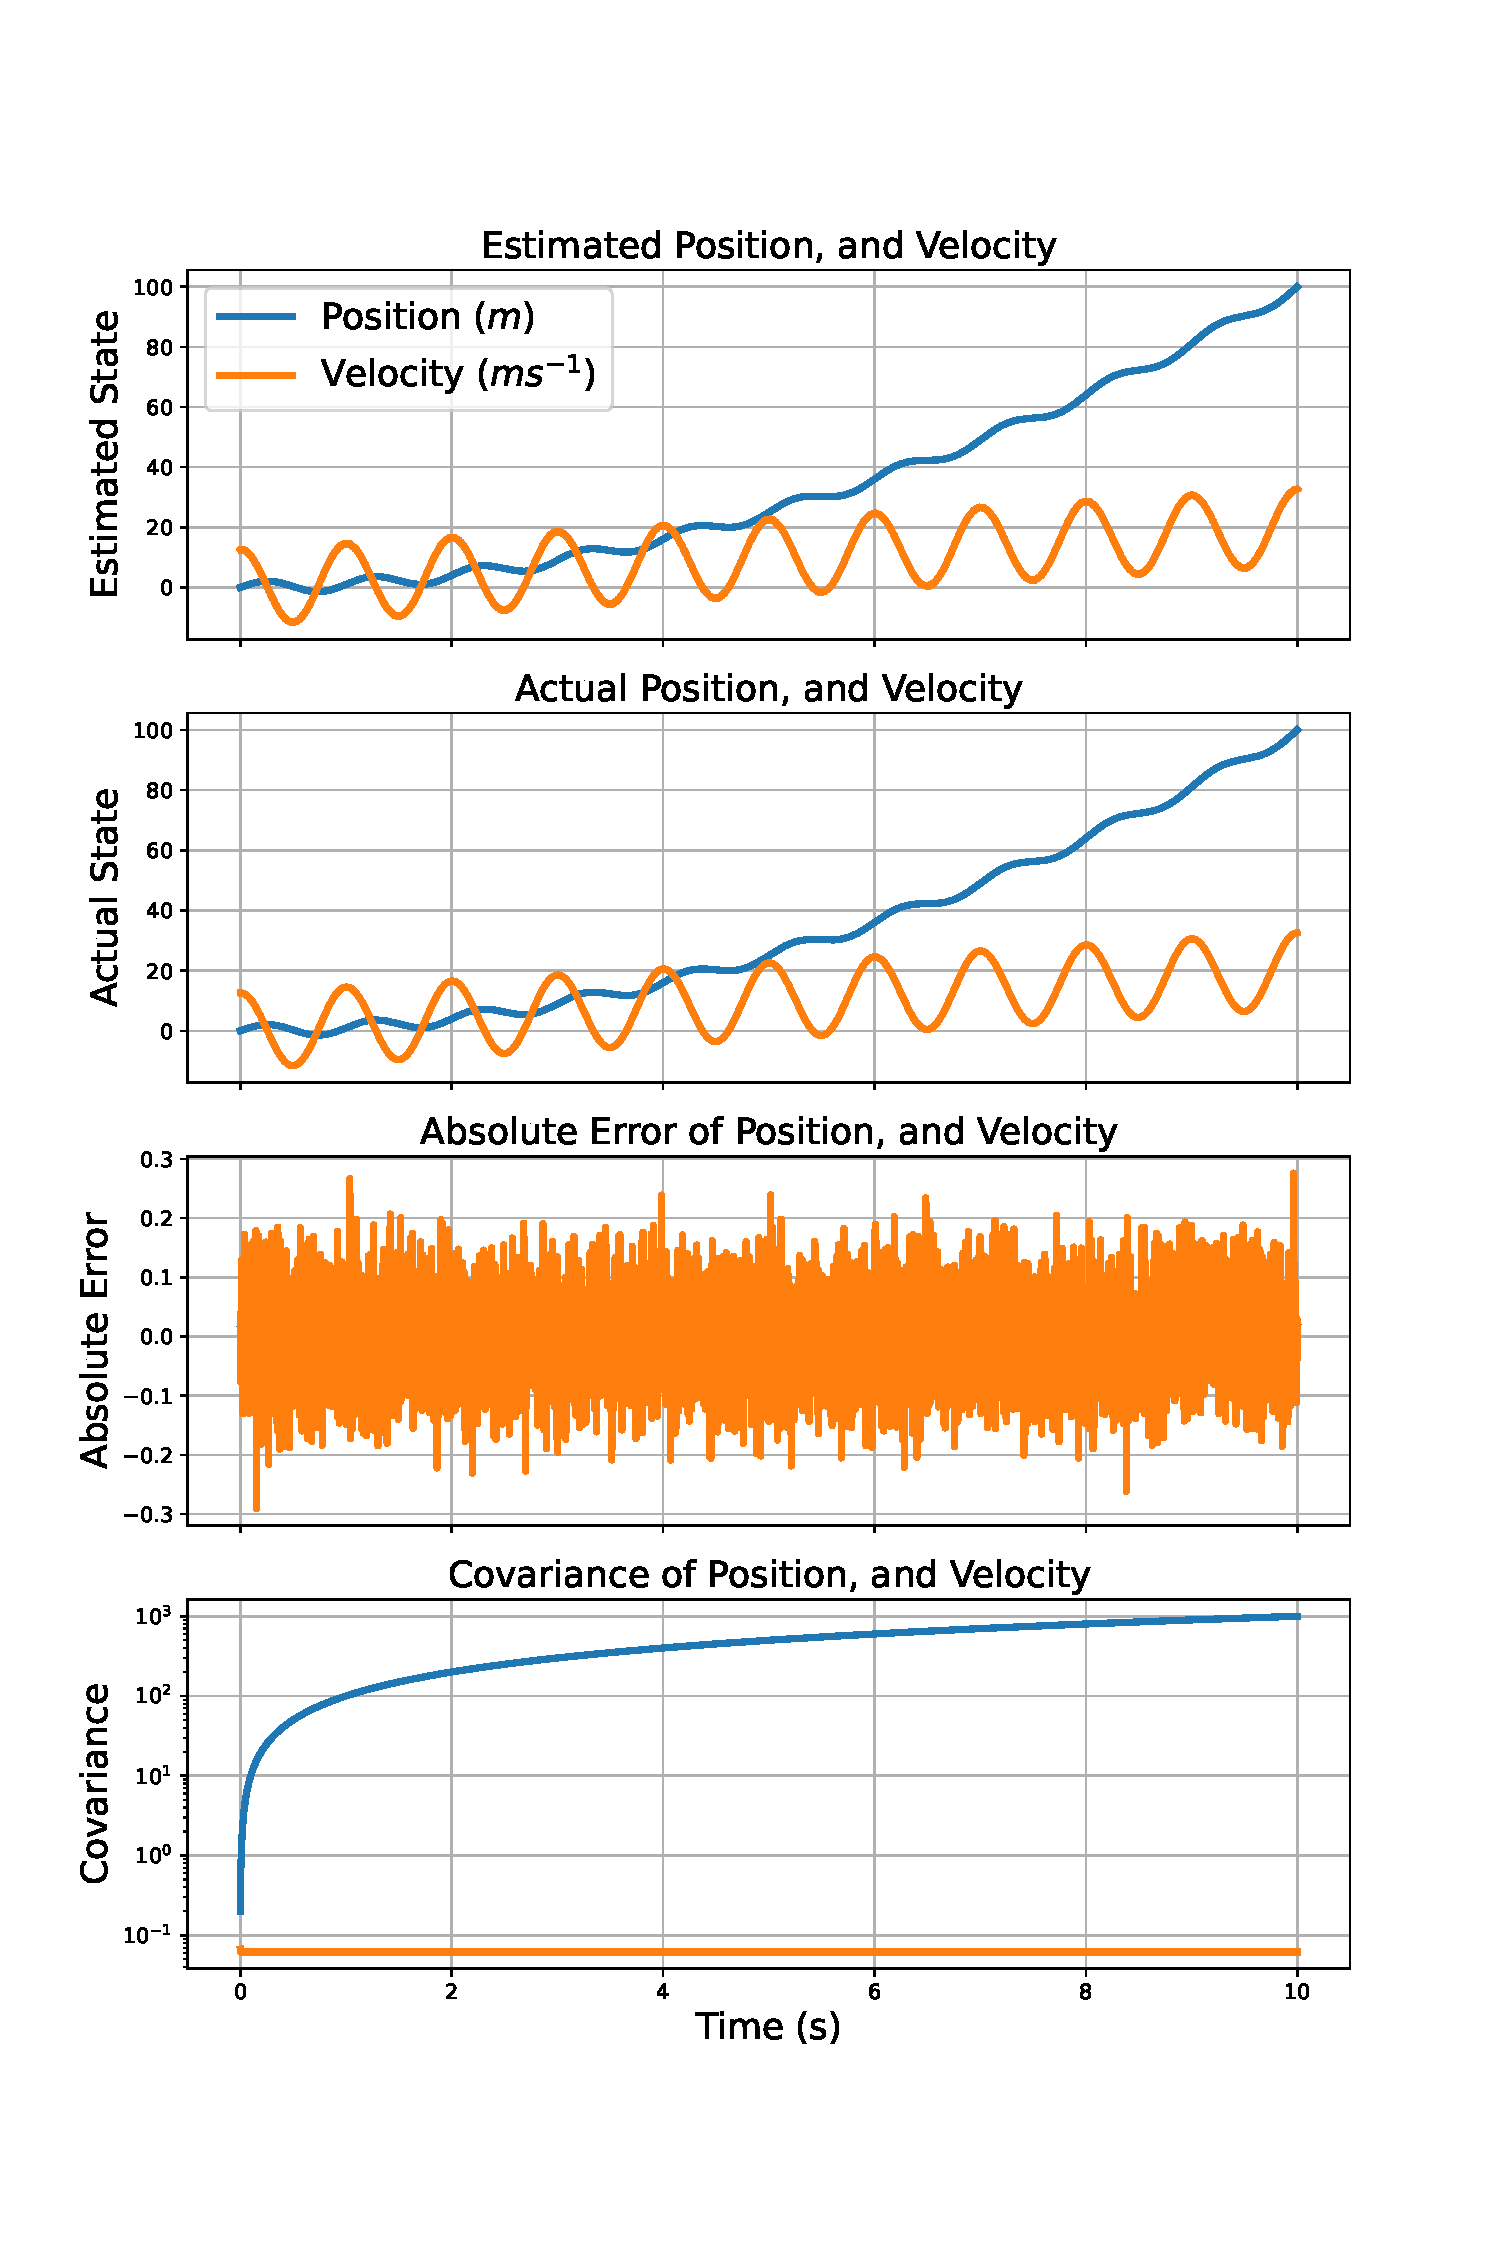
\includegraphics[height=0.8\textheight]{1d-velocity.pdf}
	
	\caption{Here we see the estimate of the state continue to be fairly accurate, even when faced with an unconstrained motion in the positive direction.}
	\label{1d_velocity_fig}
\end{figure}

The final scenario is that of a three-dimensional body rocking backwards and forwards on all three axes. This also shows decent performance, which we can see in figure \ref{3d_orient_fig}. The error is low, and more importantly stays low (i.e.\@ doesn't run off to infinity).

\begin{figure}[thp]
	\centering
	
	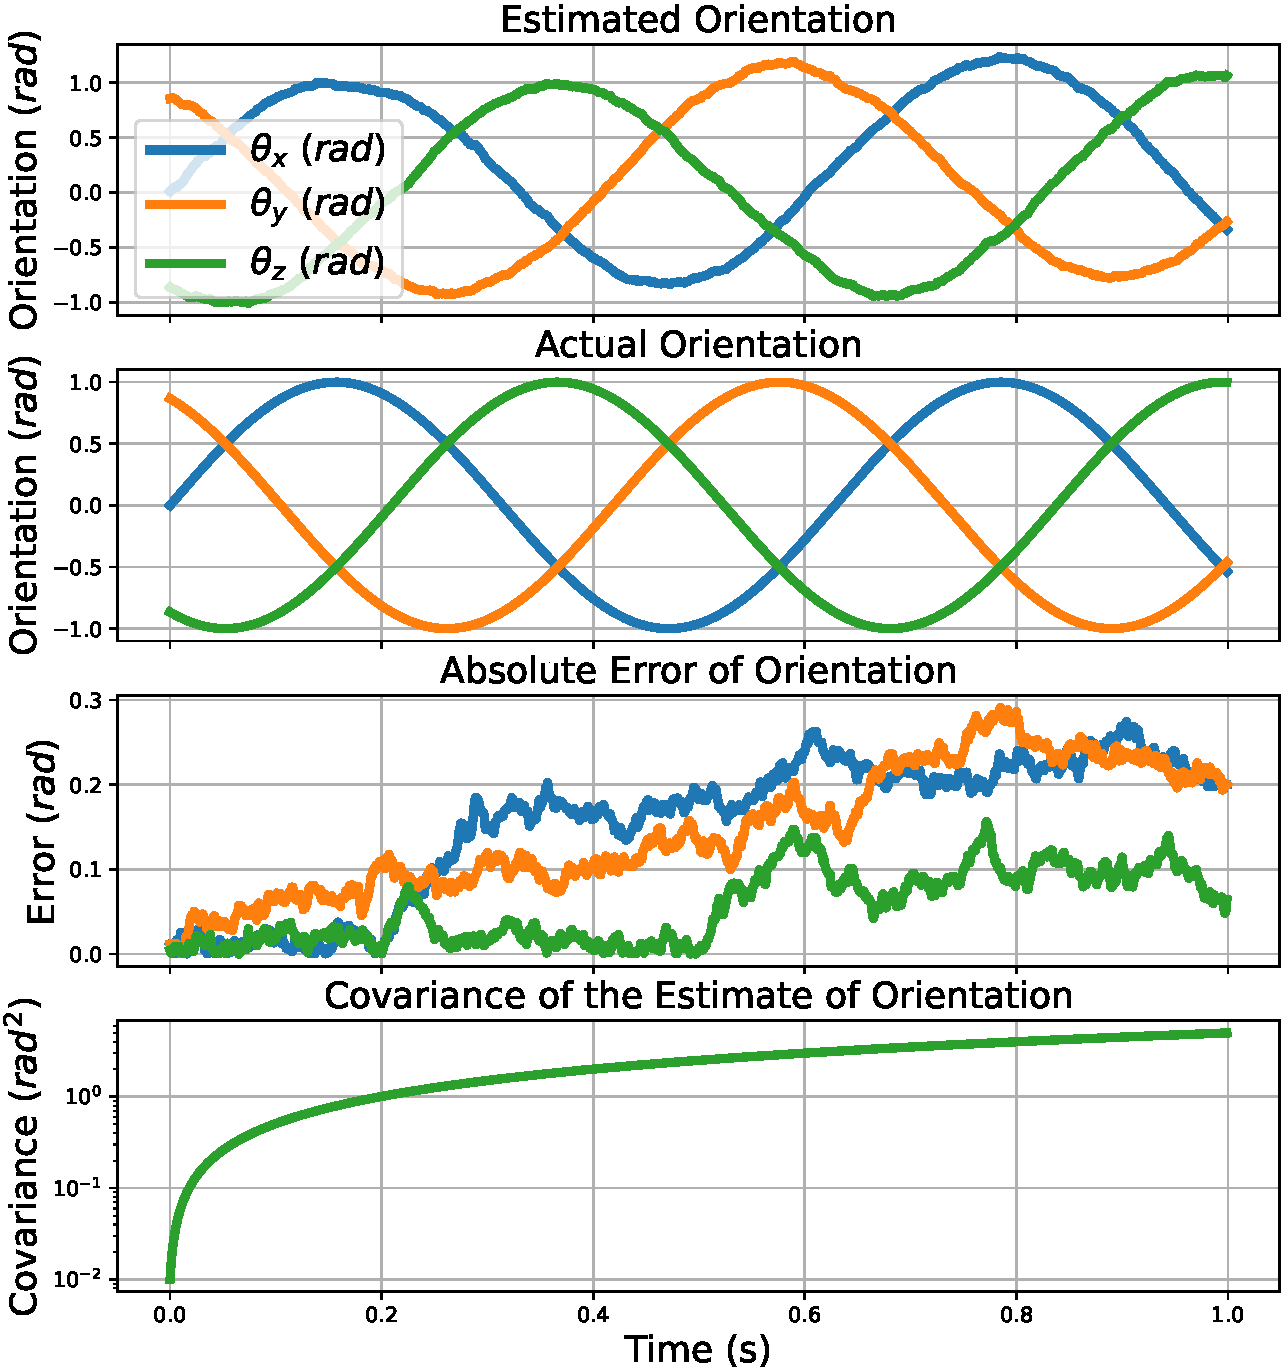
\includegraphics[width=\textwidth]{3d-orientation.pdf}
	
	\caption{A decent estimate of the orientation given noisy data. The covariance grows slowly.}
	\label{3d_orient_fig}
\end{figure}

From this we can also demonstrate how sensor and model noise affect the accuracy of the orientation estimate. For a discrete data set, the root-mean-square is defined as the square of the average of those values squared, i.e.

\newcommand{\RMS}{\ensuremath{\mathit{RMS}}} % <dme> oh, oops - you use RMS once in maths. The command is a bit of overkill then!! :-) Still, the mathit fixes the inter-letter spacing.
\begin{equation}
	x_\RMS = \sqrt{{1 \over n}(x_1^2 + x_2^2 + \dots + x_n^2)}
\end{equation}

If we run multiple iterations of the three dimensional scenario, altering the amount of noise added to the measurements and system each time, we can calculate the RMS of the error values and plot that against that noise figure, as shown in figure \ref{3d_rms_fig}.

\begin{figure}[tp]
	\centering
	
	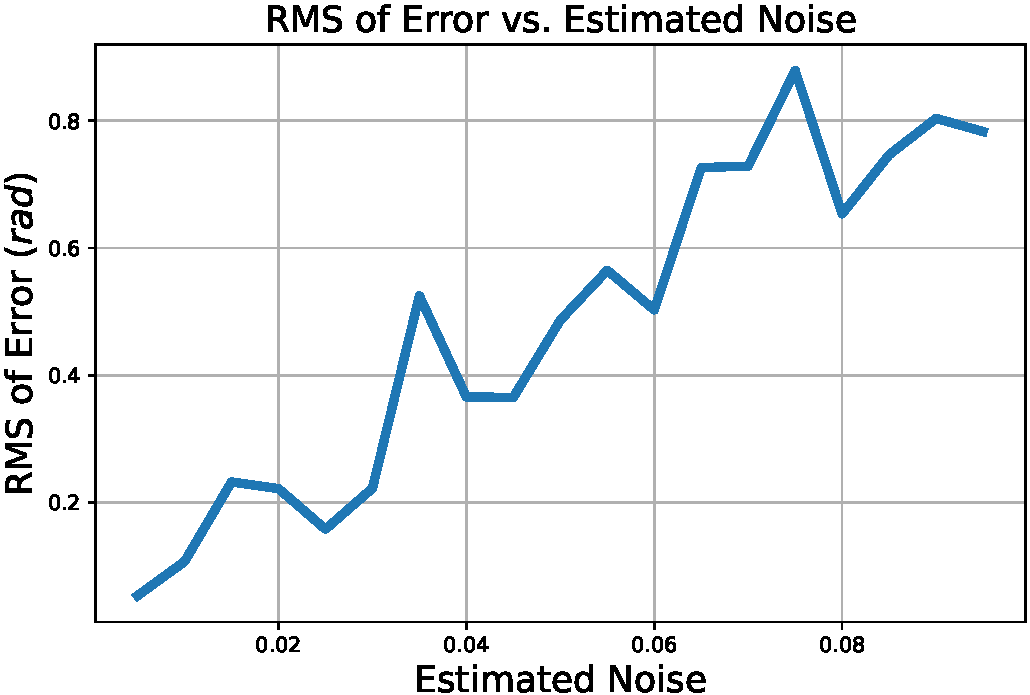
\includegraphics[width=\textwidth]{3d-rms.pdf}
	
	\caption{A plot showing the average error increasing as the amount of noise increases. The growth is approximately linear.}
	
	\label{3d_rms_fig}
\end{figure}

Here we see linear growth (with some noise)---as we make the simulated sensors more noisy the quality of the output goes down. We can see the effect of this noise in figure~\ref{3d_noise_fig}---where the noise is five times greater than in figure~\ref{3d_orient_fig}.

\begin{figure}[thp]
	\centering
	
	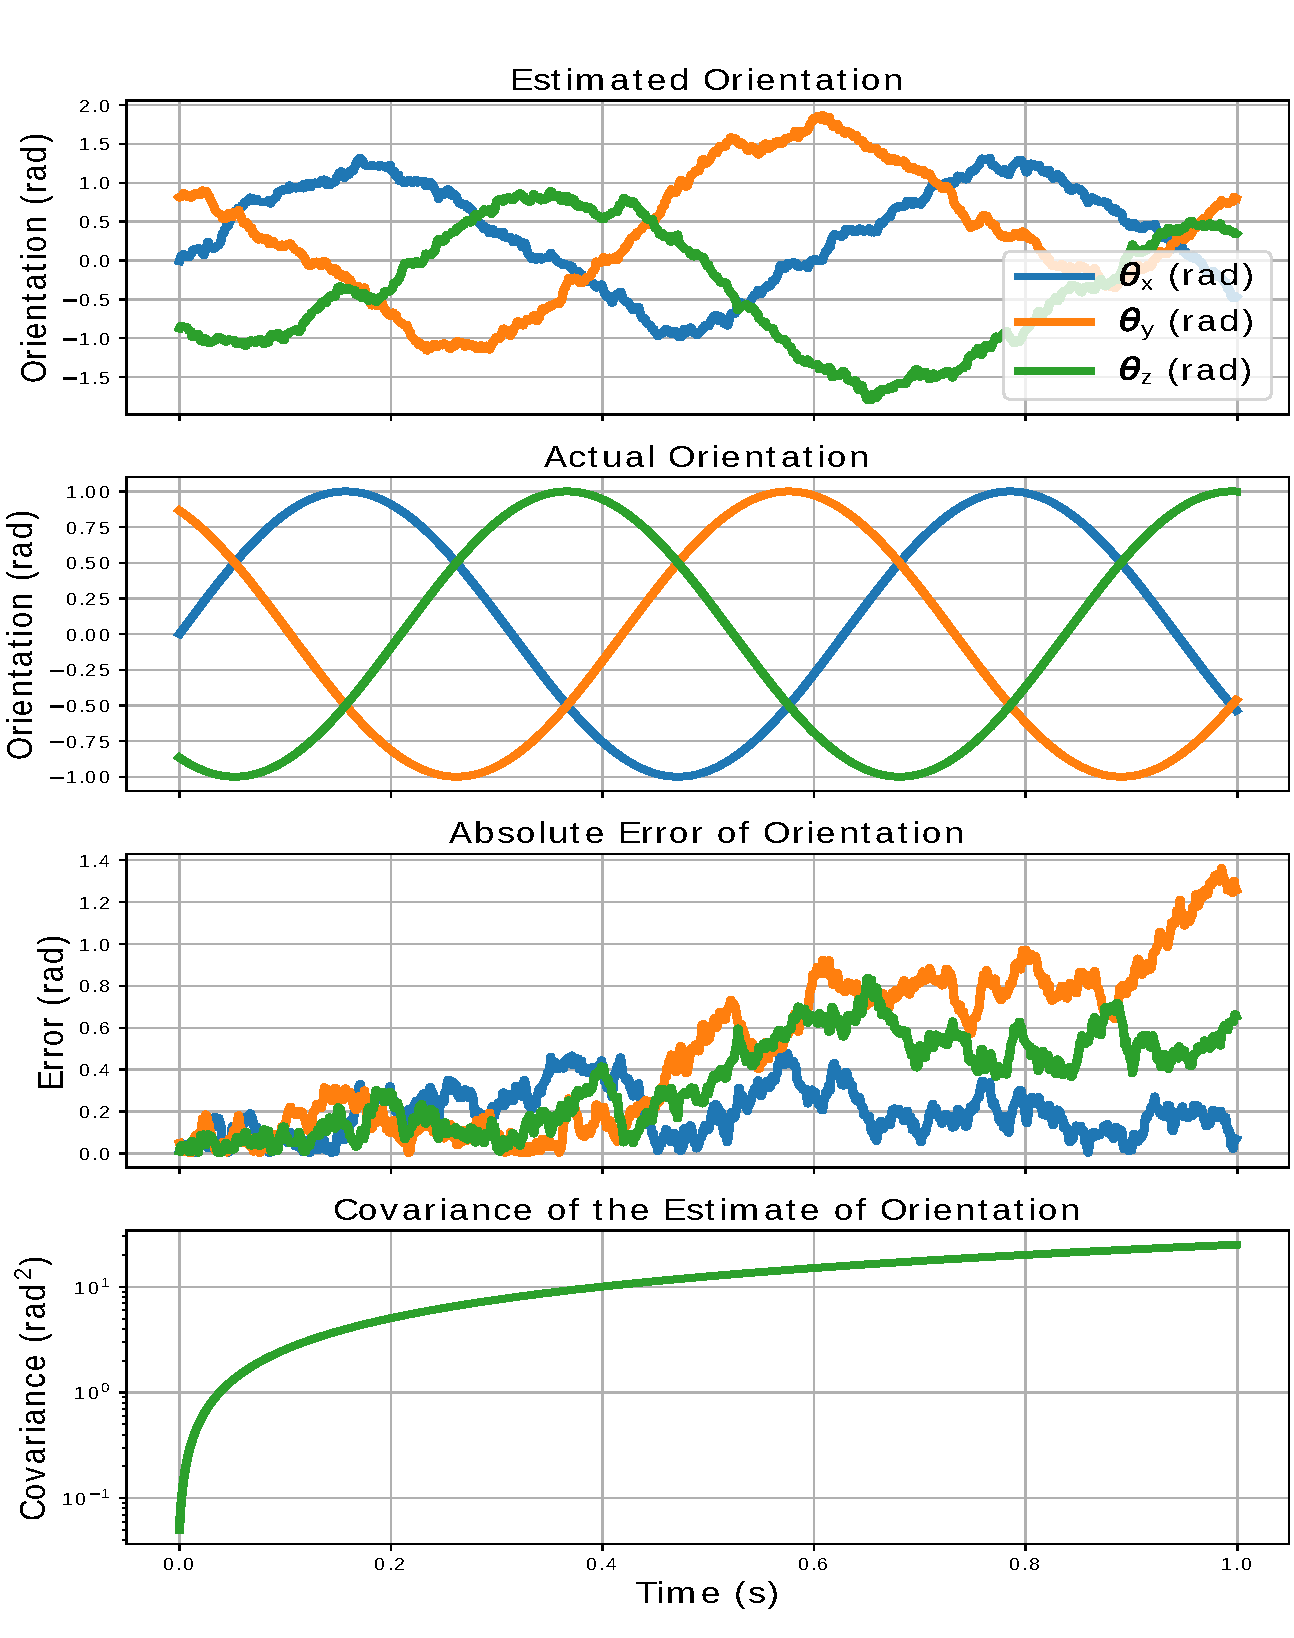
\includegraphics[height=0.8\textheight]{3d-orientation-noisy.pdf}
	
	\caption{The filter performing much worse---but the error is still bounded---and the shape of the periodic curves does approximately match reality.}
	\label{3d_noise_fig}
\end{figure}

\subsection{Verilog Implementation}

As can be seen in \ref{recursion_space}, the amount of Verilog code required to perform a moderately complicated mathematical operation is quite vast.

The $4\times4$ code I show could be written by hand fairly easily, however this would not be possible for the $12\times12$ matrix required for three dimensions each of orientation, acceleration, angular velocity, and the magnetic field vector---even a $9\times9$ version took up 40 slides in Beamer.

The solution is to automatically generate the Verilog code in software---this is the approach I used for the code in \ref{recursion_space}. This is not a trivial task but it is significantly easier to write a few hundred lines of Python than 20 KiB of Verilog.

So far, I have a reliable tool to generate the Verilog for calculating the determinant of arbitrarily sized matrices (with the maximum size specified when the Verilog is generated). I have also created a testbench module and associated Python script to confirm that it is, in fact, reliable.
\notedme{Add text describing how you're checking the result is reliable. You proceed to talk about 8-bit and 16-bit number representations without having let the reader know why this sort of size selection of numbers is necessary and/or useful.}

The testbench model gives the following output when the matrix values are between -10 and +10, and all numbers are 8 bits long, for $2\times2$ matrices. It outputs information when the result from Icarus differs from what Python's \lstinline|numpy| library expects. Here we can see the module failing occasionally due to integer overflow\footnote{Note that in each case, if we flip all the bits in the numbers labelled ``Parsed matrix determinant" and add one, then the number will be (when interpreted as a two's compliment number) the same as the number labelled ``Icarus determinant"} somewhere in the operation, due to the size of the numbers:

\lstinputlisting[numbers=none, backgroundcolor=\color{white}]{testbench-output-28.txt}

With 16-bit numbers, all 1000 runs for the $2\times2$ matrices succeed. For a $6\times6$ matrix, 24-bit numbers are needed. If the range of matrix values is increased to -100 to 100 then 48 bits are required for a $6\times6$ matrix, and 16 bits are required for a simple $2\times2$ matrix. For a $12\times12$ matrix with numbers ranging from 0 to 10, similar to what I would expect to see in a Kalman filter, 128-bit numbers are required, 64 whole bits, and 64 decimal bits.

We can see this in the figures \ref{full_heat} and \ref{full_sfc}. What we can see is that the integer width needs to be sufficient to prevent overflow, and no more, i.e.\@ there is no benefit to using larger integer components. This is in contrast to the decimal component, where we see that increasing that reduces error linearly, until about 56 bits, where it starts to flatten out.

\begin{figure}[thp]
	\centering
	
	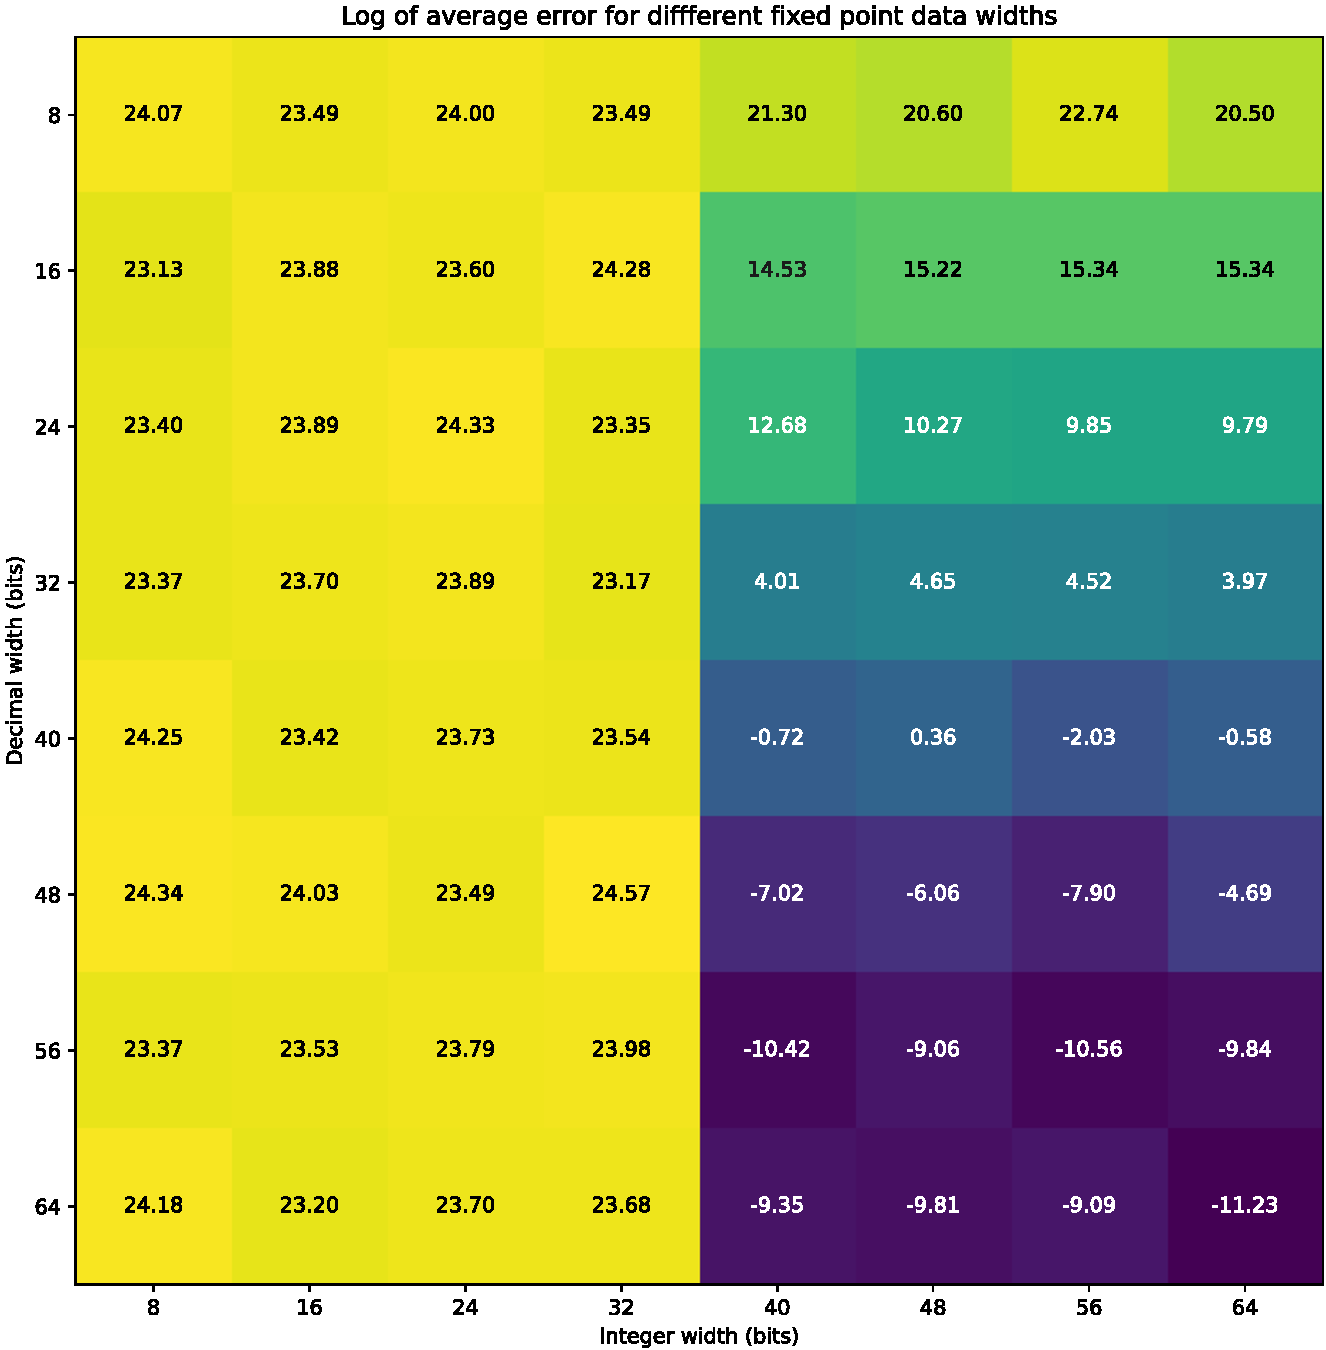
\includegraphics[width=\textwidth]{heatmap_full.pdf}
	
	\caption{A heat-map of the base 10 $\log$ of the average error of the determinant (when compared to the result from \lstinline|numpy|), after 10 runs for a $12 \times 12$ matrix. Darker colours (smaller numbers) are better.}
	\label{full_heat}
\end{figure}

\begin{figure}[thp]
	\centering
	
	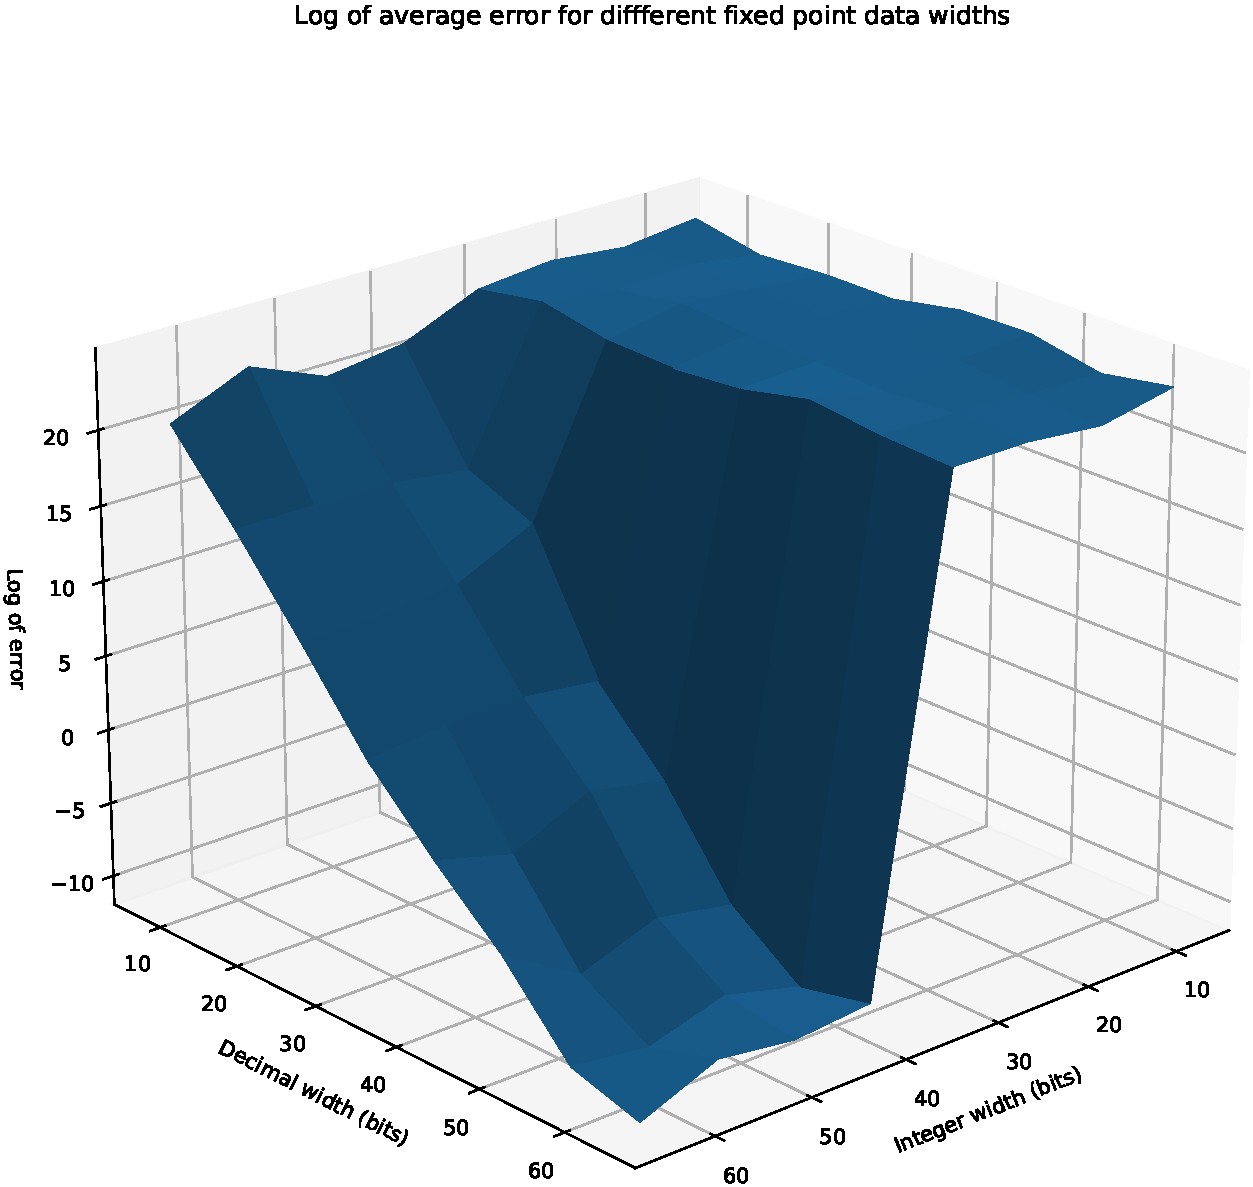
\includegraphics[width=\textwidth]{sfc_plot_full.pdf}
	
	\caption{The same plot as above, but as a 3D surface plot as opposed to a heat-map. The steep gradient at around a 40-bit wide integer component is very visible here. Lower is better.}
	\label{full_sfc}
\end{figure}

My first implementation of the matrix operations was using the naive algorithms, as described in section \ref{naive}. This implementation worked, however when it came to simulating the Verilog, both the determinant, and even more so the inverse took a very long time for the $12 \times 12$ case. I had estimated that simulating the $12 \times 12$ inverse would take about a whole day, and also be far too time consuming to implement in practice. As a result of this, I turned to the LU decomposition, as discussed in section \ref{lu}. Due to time constraints, I was only to implement the ``half-naive'' inverse, however this alone made a huge difference: The simulation time dropped to 10 minutes---and the predicted performance wasn't too bad---about 2.5 million clock cycles to complete an operation. On a 100 MHz FPGA this could do 40 operations per second. Since there is only one inverse per Kalman Filter cycle, and the inverse operation takes the longest by far of all of the operations, I would expect to be able to run about 40 Kalman filter cycles per second, which would be sufficient for real time operation. This is not ideal however, so a future work goal would to implement the full use of the LU decomposition for the matrix inverse. This would reduce the runtime from $\mathcal{O}(n^5)$ to $\mathcal{O}(n^3)$, i.e. for a $12 \times 12$ matrix it would take 144 times less \notedme{a bit confusingly expressed here, although the next sentence is clear}. That would mean only around 20,000 clock cycles, or over 5,500 Kalman Filter cycles per second. This is a huge improvement.

\subsubsection{Synthesis and Implementation}

Due to time constraints I was not in a position to put a final bitstream on an FPGA, however I was able to synthesize it, and place and route it, based on the target device being a Xilinx Artix-7 XC7A100TCSG324, shown in figure~\ref{tim_xilinx}.

\begin{figure}[thp]
	\centering
	
	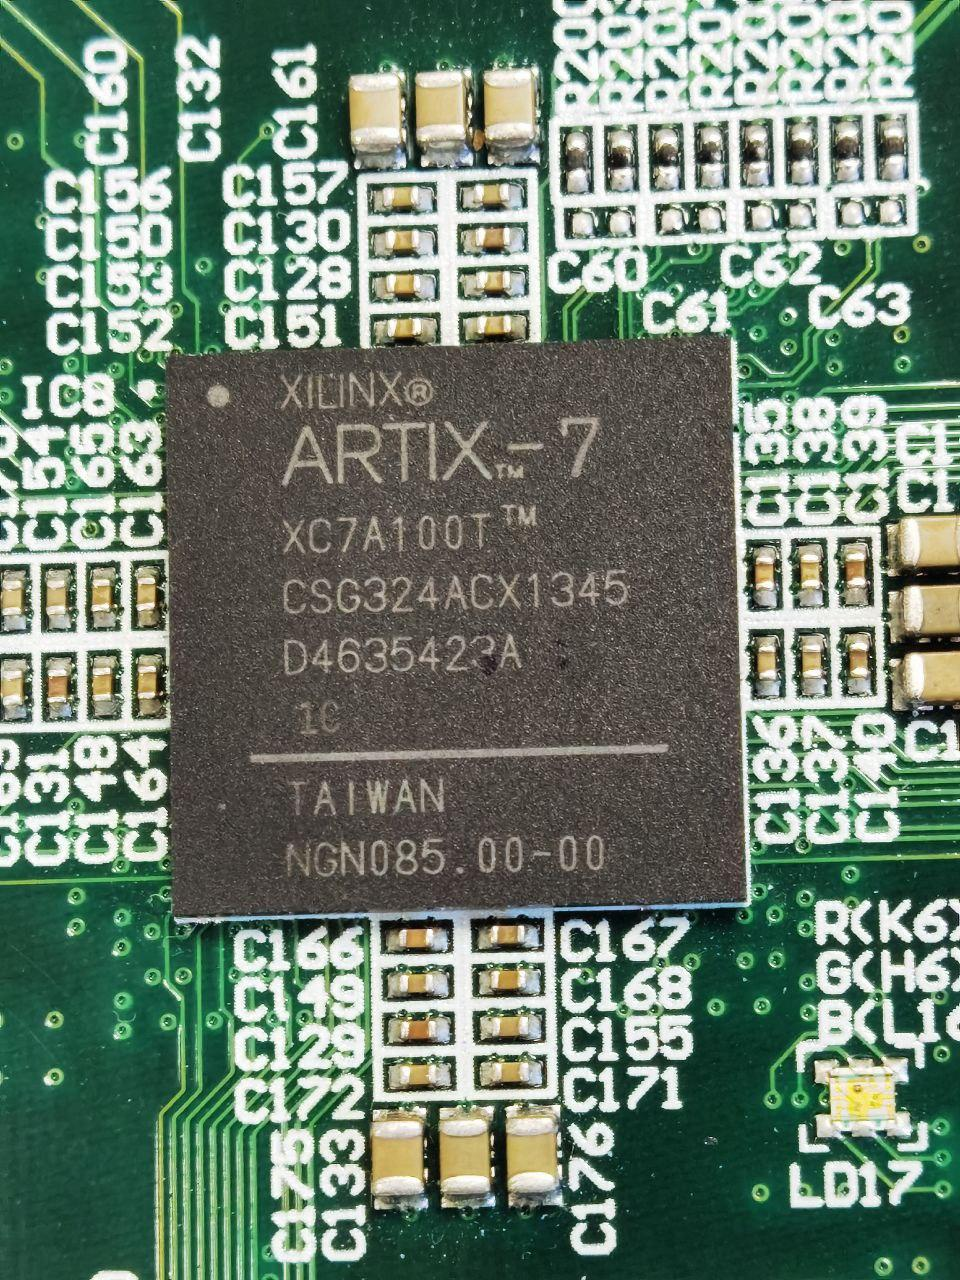
\includegraphics[width=\textwidth]{tim_xilinx.jpg}
	
	\caption{The sort of FPGA I would target for this project.}
	\label{tim_xilinx}
\end{figure}

This FPGA has 101,440 logic cells (look up tables), and 240 DSP slices (multiplier units), which should be sufficient for the purposes of this project. A development board with this FPGA on it costs around \$129.00 USD, which is entirely reasonable. Of course this would not be acceptable for a chip to be included in a phone, however if I was to actually manufacture this chip it would be fabricated to an actual dedicated chip (an application specific integrated circuit), which would be much cheaper if manufactured in volume.

\section{Future Work}

Certain specific tasks that could be done in future include

\begin{itemize}
	\item Have the matrix operations actually make a Kalman filter, and interface it with sensors.
	\item Change the matrix inverse module to directly use the matrix LU module.
\end{itemize}

\notedme{Can you put in a conclusion? It might be nice to synthesise (in the knowledge sense, not the HDL sense) where you got to in the project, e.g., where the unexpected difficulties arose. I feel that you made excellent progress, but (as is usually the case) had to diverge from your original plan due to various unforeseen complexities and issues. You've then turned the project around to produce some really good thorough results, such as the heatmap+plot of precision and accuracy tradeoffs, and quantifying the value of the LRU replacement algorithms.}

\printbibliography

% Activate the appendix
% from now on sections are numerated with capital letters
\appendix

\renewcommand{\thesection}{Appendix \Alph{section}}

\section{Basic CPU in Verilog}
\label{verilog_cpu}

\lstinputlisting[language=Verilog]{cpu-include.v}

\section{Example of Recursion in Time}
\label{recursion_time}

\lstinputlisting[language=Python]{recursion-time.py}

\section{Example of Recursion in Space}
\label{recursion_space}

\lstinputlisting[language=Verilog]{recursion-space.v}

\end{document}